% assignment_5.text - Assignment 5 for Data Fusion class (Fall 2014)
% Chanmann Lim - October 2014

\documentclass[a4paper]{article}

\usepackage[margin=1 in]{geometry}
\usepackage{amsmath}
\usepackage{listings}
\usepackage{graphicx}

\everymath{\displaystyle}

\begin{document}
\title{CS 8790: Solution to assignment 5}
\author{Chanmann Lim}
\date{October 20, 2014}
\maketitle

\subsection*{Report:} ~\\
\indent The sensor's state is a 3D measurement of the position of the target however the observations are obtained in lower dimensions (1D and 2D) with respective transformation matrix $H$. \\
\\
\indent In the provided data file comes with a mixture of those 1D and 2D observations and only differentiated by the dimensionality encoded at the beginning of each measurement. Thus, reading the dimension value(integer) is crucial to determine the numbers of subsequence data(floats) to be extracted to get an observations. In the case that the observation is one dimensional the number of float value to read is $1+1+3=5$, one value for mean $z$, one for covariance $R$ and three for the transformation matrix $H$. For 2 dimensional observation, the numbers of value to read from the data file is $2+3+6=11$, two for the mean, three for the covariance and 6 for the transformation matrix.\\
\\
\indent After obtaining the observation, we can initialize the filter with the mean $x$ equals to zero and covariance $P$ to a large number then combine them together using the below fusion equation until all observations are fused.\\
\begin{align*}
x = \begin{bmatrix}
		0   \\  0   \\   0
	\end{bmatrix}, 
P = \begin{bmatrix}
		100000000   &  0   &   0 \\
		0   &  100000000   &   0 \\
		0   &  0   &   100000000
	\end{bmatrix}
\end{align*}

\paragraph{1. } The final mean $x$ and the new covariance $P$ are computed using innovation form of the fusion equation:
\begin{align*}
x_{new} &= x + W(z-x) \\
P_{new} &= P - WSW^{T}
\end{align*}
where
\begin{align*}
S = R + P \\
W = PS^{-1}
\end{align*}
\begin{align*}
x_{final} = 
	\begin{bmatrix}
		12.895992   \\  130.398454   \\   23.494780
	\end{bmatrix}
\end{align*}
\begin{align*}
Square \; root \; of \; P_{final} = 
	\begin{bmatrix}
        0.002755   &    0.001226   &    0.000953 \\
      	0.001226   &    0.003708   &    0.002179 \\
      	0.000953   &    0.002179   &    0.004934
	\end{bmatrix}
\end{align*}

\paragraph{2. } Plots:\\
\\
Normalized innovations:\\
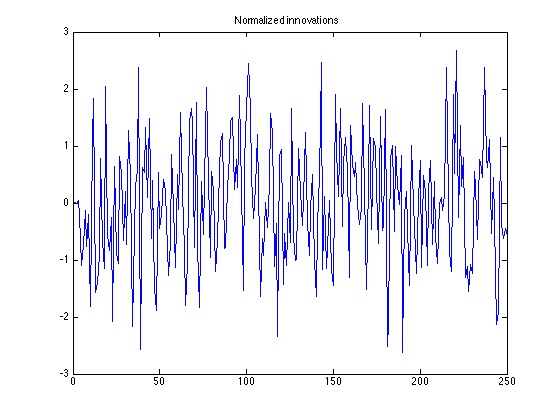
\includegraphics[scale=.8]{normalized_innovations.png}\\
Randn:\\
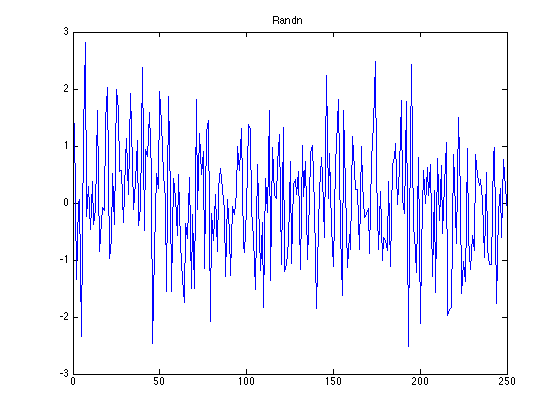
\includegraphics[scale=.8]{randn.png}

\newpage
\subsection*{Appendix:}
\lstinputlisting[language=Matlab, title=\lstname, basicstyle=\footnotesize]{assignment_5.m}
\lstinputlisting[language=Matlab, title=\lstname, basicstyle=\footnotesize]{getObservation.m}
\lstinputlisting[language=Matlab, title=\lstname, basicstyle=\footnotesize]{update.m}

\end{document}